\section{Code source}
\subsection{Fonction $\frac{1-z^{-1}}{2}$}
\lstinputlisting[caption={Code source pour l'exercice 3 fonction $\frac{1-z^{-1}}{2}$}, label=lst:label, language=Octave]{src/ex3-1.m}

\subsection{Fonction $\frac{1+z^{-1}}{2}$}
\lstinputlisting[caption={Code source pour l'exercice 3 fonction $\frac{1+z^{-1}}{2}$}, label=lst:label, language=Octave]{src/ex3-2.m}

\subsection{Fonction $\frac{1-z^{-2}}{2}$}
\lstinputlisting[caption={Code source pour l'exercice 3 fonction $\frac{1-z^{-2}}{2}$}, label=lst:label, language=Octave]{src/ex3-3.m}

\subsection{Fonction $\frac{2z^{-1}}{2-z^{-1}}$}
\lstinputlisting[caption={Code source pour l'exercice 3 fonction $\frac{2z^{-1}}{2-z^{-1}}$}, label=lst:label, language=Octave]{src/ex3-4.m}

\subsection{Fonction $\frac{2z^{-1}-z^{-5}}{2-z^{-1}}$}
\lstinputlisting[caption={Code source pour l'exercice 3 fonction $\frac{2z^{-1}-z^{-5}}{2-z^{-1}}$}, label=lst:label, language=Octave]{src/ex3-5.m}

\section{Résultats obtenus}
\subsection{Fonction $\frac{1-z^{-1}}{2}$}
Nous commençons par afficher le diagramme de gain en décibel ()ainsi que le diagramme de phase en radians () pour déterminer la nature du filtre représenté par cette fonction de transfert.
%\begin{figure}
%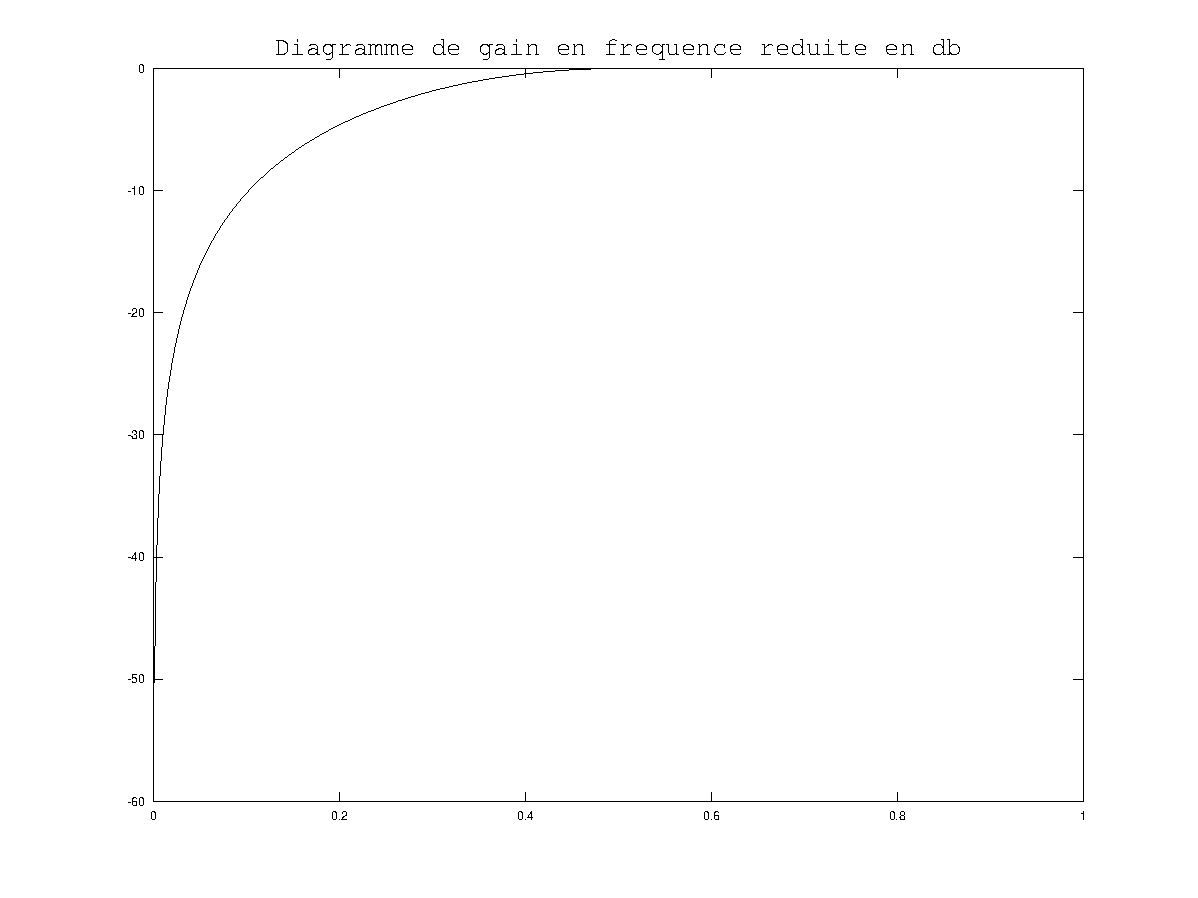
\includegraphics{f1Gain}
%\end{figure}
salut
%$\frac{1-z^{-1}}{2}$
salut
